\documentclass[11pt,a4paper]{article}
\usepackage[utf8]{inputenc}
\usepackage[hmargin=2.0cm,vmargin=2.5cm,bindingoffset=0.5cm]{geometry}
\usepackage{amsfonts}
\usepackage{amsmath,amsthm,amssymb}
\usepackage{hyperref}
\usepackage{graphicx}
\usepackage{setspace}
\doublespacing
\usepackage{tikz}
\usepackage{mathtools}
\DeclarePairedDelimiter\ceil{\lceil}{\rceil}
\DeclarePairedDelimiter\floor{\lfloor}{\rfloor}
%\usepackage{float}
\usepackage{placeins}
\usepackage{diagbox}
\newtheorem{thm}{Theorem}
\usepackage{subcaption}
\interfootnotelinepenalty=10000
%\usepackage{subfigure}
\usepackage[english]{babel}
\author{Mohit}
\title{Transition between two equilibrium configurations}
\begin{document}

\maketitle

\section{Introduction}
We would be studying an optimization problem in a classical non-equilibrium problem. Our model under consideration would be a Langevin particle coupled to a heat bath. We would be driving the system from one equilibrium state to another through a certain protocol. Usually, it takes certain time for this transition between two different equilibrium configurations of the system. The question is can we reduce this transition time to arbitrary small?

To get some intuition, let's consider a textbook example of expansion of gas in a cylinder with a piston. We start off in an equilibrium configuration, and then we increase the height of cylinder by pulling its' piston. On one hand, if the system is driven slow enough, then the system takes infinite time in reaching the new equilibrium configuration. On the other hand, if the system is driven really fast, then the system is in non-equilibrium and it usually takes some time (characteristic relaxation time $\tau$) to relax  to the new equilibrium configuration.

Does there exist a clever protocol in which transition time is arbitrary small? In other words, can we beat the system's relaxation time $\tau$? The answer is yes given in \cite{martinez2016engineered} .




Inspired by their results, we study Langevin dynamics when spring stiffness is changed through a linear ramp. I would start off by writing down general Langevin equation of a particle in a harmonic potential with a constant spring stiffness. To gain some insights into the physics of dissipation and noise, we would take different cases: random walker (affect of noise), tired walker (affect of dissipation) and overdamped Brownian particle (affect of noise and dissipation together). Once we understand the problem with constant spring stiffness, we study the transition between two equilibrium configuration (defined by two different values of spring stiffness) as spring stiffness is  changed linearly.
\section{Definition of thermal equilibrium}
Before we start our study, we should define what it means for a particle to be in  thermal equilibrium. We would call a particle to be in equilibrium if following conditions are met  in a particular configuration/state:
\begin{itemize}
\item For each degree of freedom, the average kinetic $K$ and potential $V$  energy will follow equipartition theorem, i.e  $\langle K \rangle$ = $\langle V \rangle = k_B T/2$. In our model of  overdamped Brownian particle in Harmonic potential, there is no kinetic energy. Hence, we will get   $  \langle E \rangle= \langle V \rangle = \kappa \langle x^2 /2\rangle = k_B T/2$, where $\kappa$ and $T$ is the spring constant and temperature, respectively.
\item Physical properties of the system should be time-independent. For example, in models under our consideration, mean and second raw moment of position, and probability density of position would be constant in time when the particle has relaxed to equilibrium \footnote{Note once the probability density relaxes to that of Boltzmann distribution, then equipartition theorem is guaranteed to hold.}.
\end{itemize}


\section{Langevin dynamics}

Let's write the general equation of a particle under a harmonic potential of stiffness $k$ and dissipation $\Gamma$:
\begin{equation}
m \ddot{x}= -k x -\Gamma \dot{x} + \xi(t)
\end{equation}

\begin{equation}
\langle \xi(t)\rangle=0, \quad \langle \xi(t) \xi(t^{\prime}) \rangle= 2 D \delta(t- t^{\prime})
\label{moment}
\end{equation}

where $\xi(t)$ is white noise. Its' first and second raw moments are given in equation \ref{moment}.What does condition on the second moment mean? Noise for different times is uncorrelated. For the same time, we see that second moment diverges. It's chosen for analytical convenience, which is not suitable for numerical simulations. To study the Langevin equation numerically, Euler-Maruyama algorithm was used. (appendix \ref{sec.Numerics}).


We are going to consider overdamped Brownian particle where we assume $\Gamma / m \gg 1$ . Thus, we can ignore $m \ddot{x}$ term. Hence, we have 
\begin{equation}
  \dot{x}= -\dfrac{\kappa}{\gamma} x + \xi(t)
\end{equation}
where $\Gamma/m=\gamma$  and $\kappa =k/m$.

Due to our assumption, we find that here dissipation is proportional to position (rather than velocity $\dot{x}$) in equation of motion \footnote{see appendix \ref{sec.vel_dof} for model involving dissipation term proportional to velocity where we assume $\Gamma / k \gg 1$. We ignore the spring force term there.}. 

To understand the affect of noise and dissipation, we would first study two subcases: random walker (one with only noise term) and tired walker in position (the one with only dissipation term). 



\begin{figure}[!htbp]
\centering
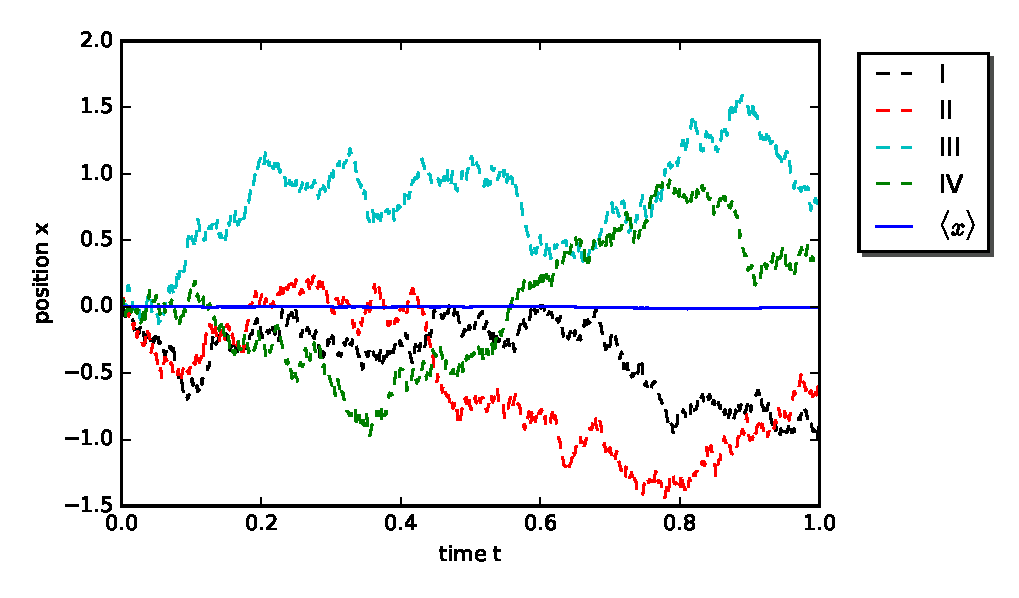
\includegraphics[scale=0.67]{x_mean.eps}
\caption{$I, II, III$ and $IV$ represent position of the random walker obtained as a function of time in first, second, third and fourth realization of noise. $<x>$ is the mean position of the random walker averaged  over 1000 realizations.}
\label{meanx}
\end{figure}


\subsection*{Random walker: affect of noise}
Langevin equation for a random walker is given by:
\begin{eqnarray}
\dot{x}=  \xi(t)
\label{rand}
\end{eqnarray}


Now, from equation \ref{rand}, we can compute the mean and variance of position. We find that mean position $\langle \Delta x\rangle=0$ (figure \ref{meanx}) and variance $\langle \Delta x ^2\rangle=2 Dt$ (figure \ref{varx}), where $\Delta x= x(t)-x(0)$. Hence, we find that random walker never relaxes to equilibrium since  $\langle \Delta x ^2\rangle$ always grows in time. 




\begin{figure}[!htbp]
\centering
\includegraphics[scale=0.67]{x_var.eps}
\caption{ Variance $\langle \Delta x ^2\rangle$ of the random walker as a function of time with $D=1/2$(dashed blue line).  Red line is the fitted line linear in time $t$.  }
\label{varx}
\end{figure}




\subsection*{Tired walker: affect of dissipation}
Now we would focus on the affect of dissipation by studying a tired walker, which follows:
\begin{equation}
\dot{x}= - \frac{\kappa}{\gamma} x 
\end{equation}
We get $x(t)=x(0) e^{-\kappa t/\gamma}$ as solution (figure \ref{meanx_tired}). It means as $t\rightarrow \infty$, position  (and velocity) of particle goes to zero no matter what is the initial position (and velocity). Here, dissipation takes away total energy of the system. 

What do we learn? On one hand, with only noise term, the variance keeps growing in time. It will perpetually stay in non-equilibrium. On the other hand, when we have only dissipation term, the particle always relaxes to zero position. The final state is in equilibrium, but it's not useful for modeling anything because average energy is zero. Hence, we will study equilibrium with both of the terms present. We will find that due to dissipation-fluctuation relationship, our system reaches equilibrium with non-zero energy.



\begin{figure}[!htbp]
\centering
\includegraphics[scale=0.67]{tired_walker.eps}
\caption{ Position of the tired walker as a function of time with $\kappa/\gamma=1$ and $x(0)=1$. Euler method was used with $\Delta t=0.01$.  }
\label{meanx_tired}
\end{figure}






\subsection*{Overdamped Brownian particle}
Now let's consider overdamped Brownian particle with both dissipation and noise terms. It follows:
\begin{equation}
\dot{x}= -\dfrac{\kappa(t)}{\gamma} x + \xi(t)
\label{eom}
\end{equation}


\subsubsection*{Constant spring stiffness}
We can solve this equation analytically when spring stiffness $\kappa(t)= \kappa$ is a constant. Then, we get: 
\begin{equation}
x(t)= x(0) e^{-\kappa t/\gamma} + \int_0^t ds  \xi(s) e^{-\kappa (t-s)/\gamma} 
\label{sol}
\end{equation}

Hence, when we average over noise to find mean position, we get $\langle x \rangle=x(0) e^{-\kappa t/\gamma}$ (figure \ref{meanx_brown}).
We see that characteristic relaxation time $\tau=\dfrac{\gamma}{\kappa}$, in which average position reduces by a factor by $e^{-1}$.


\begin{figure}[!htbp]
\centering
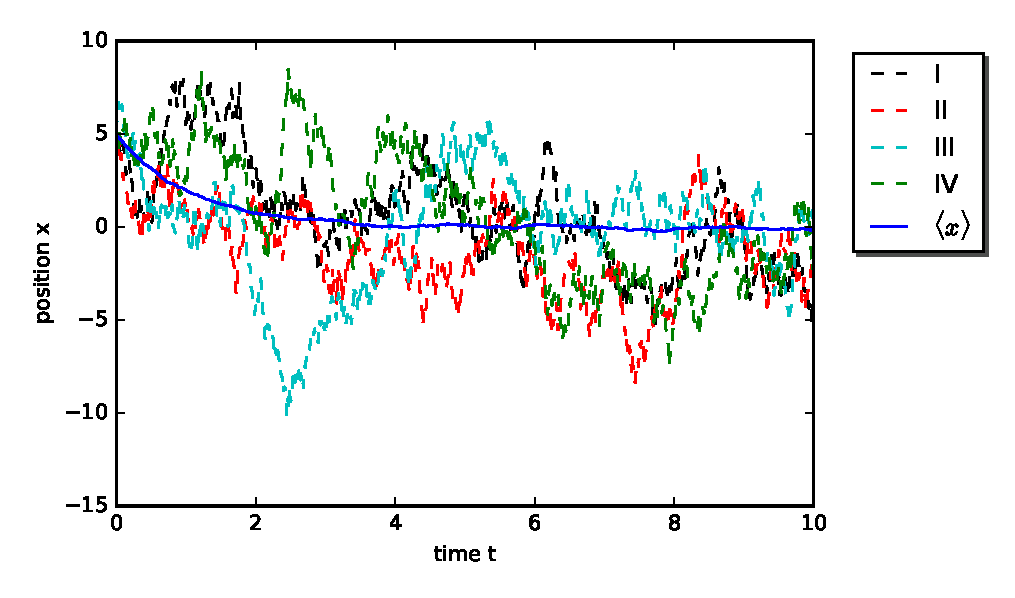
\includegraphics[scale=0.67]{x_brown_realization.eps}
\caption{ With $\kappa/\gamma=1$ and $x(0)=5$, $I, II, III$ and $IV$ represent position of the Brownian particle as a function of time in first, second, third and fourth realization of noise. $<x>$ is the mean position of the random walker averaged  over 1000 realizations . Euler-Maruyama method was used with $\Delta t=0.01$. }
\label{meanx_brown}
\end{figure}


The above equation gives us information about how position \footnote{To find velocity, we can take a time derivative of equation \ref{sol}. What's the average kinetic energy? $\langle m v^2 \rangle =0 $ since in overdamped limit, we ignore the mass term.} of particle evolves in time.
We would be interested in the position at really long time ($t\rightarrow \infty$). Since $\langle x(t\rightarrow \infty) \rangle=0$ , let's compute second raw moment \footnote{In equation \ref{var_x}, if we take $\kappa /\gamma \rightarrow 0$ so as that to get back variance of random walker, we get wrong answer. The blame should go to the step in which averaging was done of the solution from equation \ref{sol}. Before averaging, equation \ref{sol} does give us correct answer in this limit. }.
\begin{equation}
\langle x^2 (t) \rangle = \langle x^2 (0) \rangle e^{-2\kappa t/\gamma} + \dfrac{D \gamma}{\kappa}(1-e^{-2\kappa t/\gamma})
\label{var_x}
\end{equation}

\begin{figure}[!htbp]
\centering
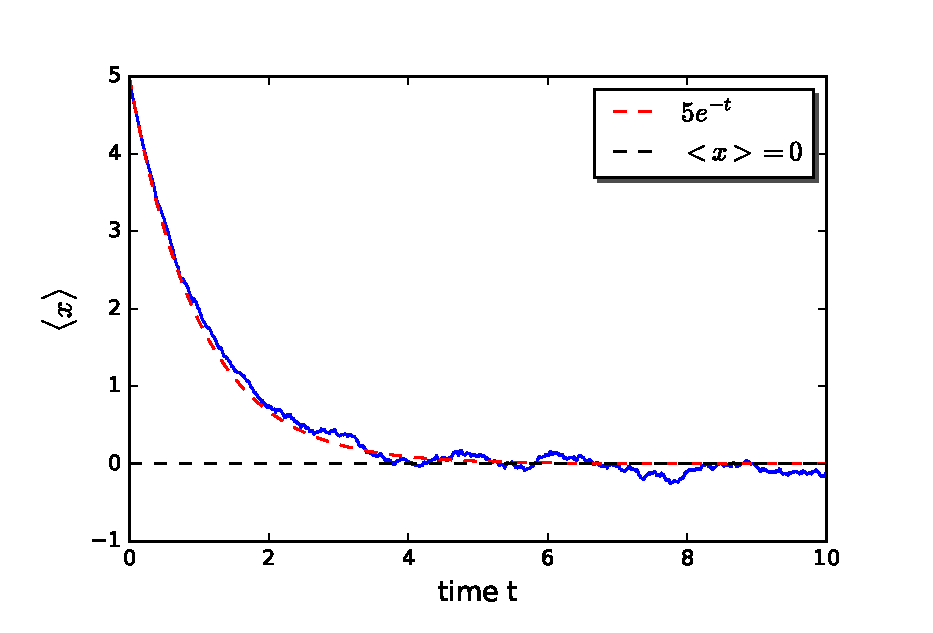
\includegraphics[scale=0.5]{x_brown_mean.eps}
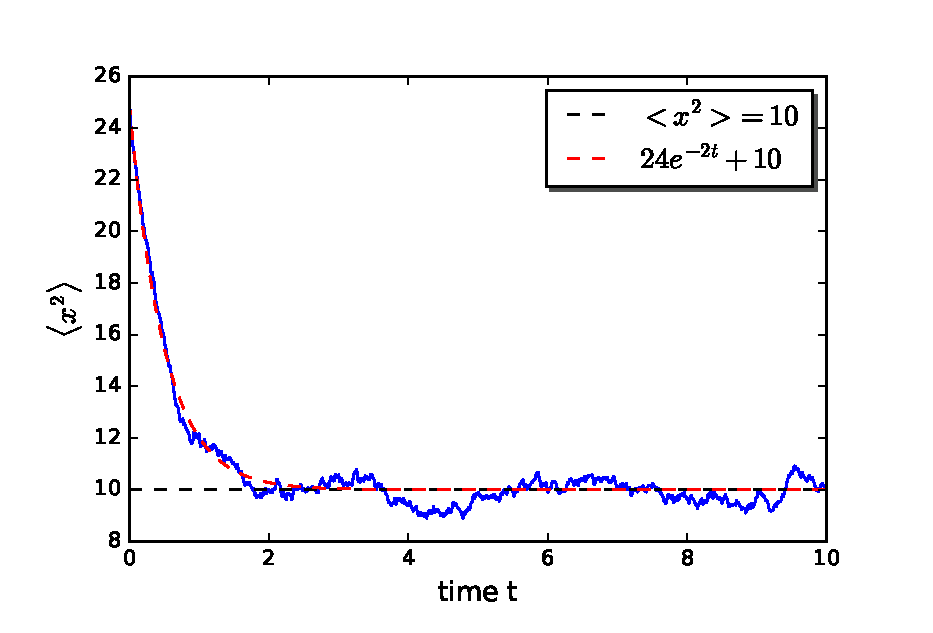
\includegraphics[scale=0.5]{x2_brown.eps}
\caption{ First $<x>$ and second $<x^2>$  raw moments of the position of the Brownian particle as a function of time with $D=10$, $\kappa/\gamma=1$ and $x(0)=5$. Euler-Maruyama method was used with $\Delta t=0.01$. We can note that physical quantities after some time starts fluctuating around their equilibrium value}
\label{varx_brown}
\end{figure}

We see that characteristic relaxation time $\tau/2=\dfrac{\gamma}{2\kappa}$, in which second raw moment reduces by a factor by $e^{-1}$.


After long time, we see that Brownian particle reaches equilibrium since $\langle x^2 (t\rightarrow \infty) \rangle$ becomes time - independent. Thus, we expect it to satisfy equipartition theorem, i.e $ \langle x^2 \rangle = k_B T/ \kappa$. This would mean that $D=k_B T/\gamma$. We obtain a fluctuation-dissipation relation in this way.

Once we have understood how an overdamped Brownian particle relaxes to equilibrium, we are ready to study our main problem: reducing transition time from one equilibrium state to another. In the next section, we will be studying dynamics when spring's stiffness is increased linearly.


%We would be studying two different cases: one with $\gamma=1$ and the other with $\gamma=10$. Relaxation time is longer in later case.
%
%\underline{$\gamma=1$} \\
%The central idea is that we would be studying transition between two equilibrium configuration defined by spring constants $\kappa(0)=1$ and $\kappa(T_f)=2$ at initial and final time, respectively. Linear ramp of spring constant (figure \ref{protocol_ramp}) is given by:
%
%\begin{equation}
%  \kappa(t)=\left\{
%  \begin{array}{@{}ll@{}}
%    1 & ,0< t <10 \\
%    1+ t/t_f & ,  10 < t \leq t_f \\
%    2 & , t_f \leq  t_f+10 \\
%  \end{array}\right.
%\end{equation}
%where $t_f$ is the time it takes for spring constant to ramp from $\kappa=1$ to $\kappa=2$. Thus, smaller the $t_f$, higher is the slope $ \dot{\kappa}=1/t_f$.  We have chosen 10 time units as the time interval that we give our particle to relax to equilibrium because in figure \ref{varx_brown}, we find that it relaxes to equilibrium before 10 time units. Hence, initially, with $\kappa(0)=1$, we give 10 time units for our Brownian particle to relax to equilibrium, and then after $t=t_f$ with $\kappa(t>t_f)=2$ , we again wait for 10 time units.
%
%\begin{figure}[!htbp]
%\centering
%\includegraphics[scale=0.67]{ramp_protocol.eps}\\
%\caption{ Ramp protocol}
%\label{protocol_ramp}
%\end{figure}
%
%Note that relaxation time for mean of position $<x>$ is  $\tau=\dfrac{\gamma}{\kappa}=1$ unit. And relaxation time for second raw moment of position $<x^2>$ is  $\tau=\dfrac{\gamma}{2\kappa}=0.5$ units. 
%When $\kappa=2$, then $\tau=0.25$. We see that even with $t_f<\tau$, then we still see that particle relaxes to equilibrium! It's very surprising, and doesn't match with Nature Physics '16 paper.
%
%
%Here are a few expectations from the numerical simulation before we can start trusting these results:
%\begin{itemize}
%\item The time it takes to relax to equilibrium should NOT depend on $N_{exp}$ and $\Delta t$. Generally speaking, $N_{exp}$ should be large enough and $\Delta t$ small enough so that our numerical results don't depend on these two parameters.
%\item All of linear ramp protocol should give the same value for $0<t<10$. This expectation is met. 
%\end{itemize}
%\begin{figure}[!htbp]
%\centering
%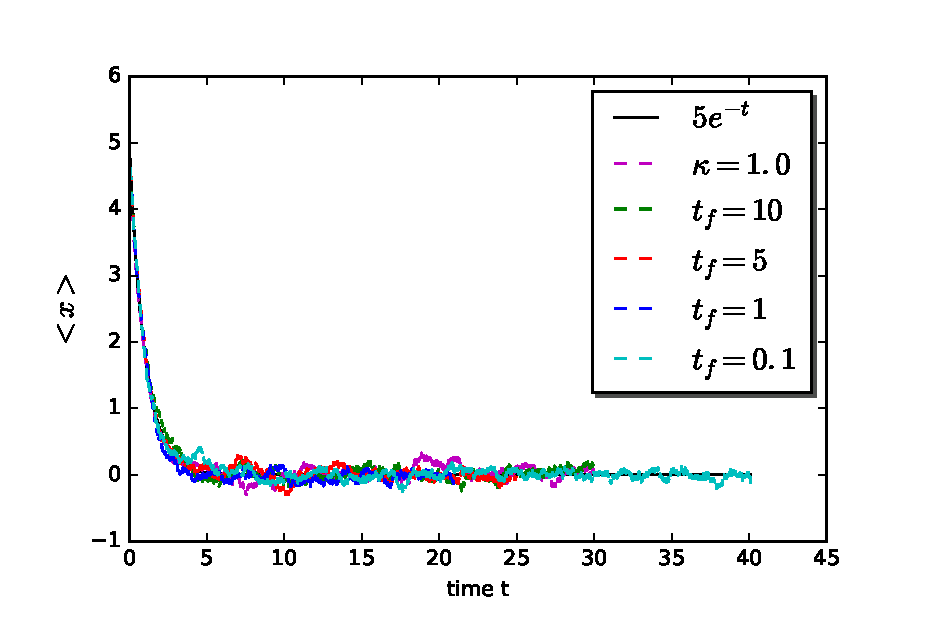
\includegraphics[scale=0.67]{ramp_mean.eps}
%\caption{ $\Delta t=0.001, D=10, \gamma=1$ and number of noise realizations $N_{exp}=1000$ over which it is averaged. For all linear protocol ramps, mean $<x>$ matches with that of mean of equation \ref{sol}}
%\label{ramp_mean}
%\end{figure}
%
%
%\begin{figure}[!htbp]
%\centering
%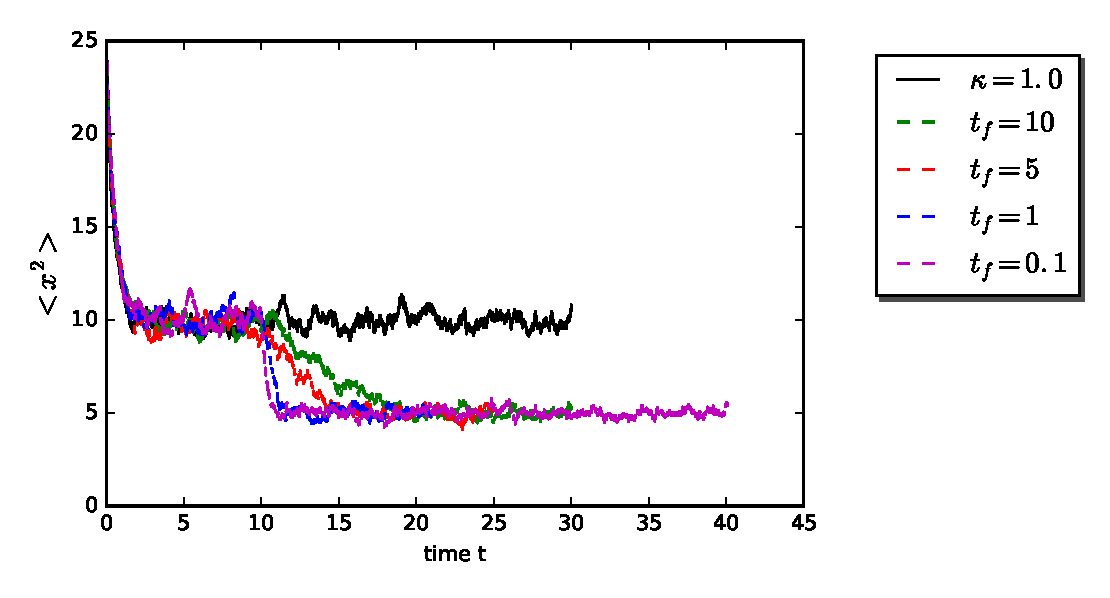
\includegraphics[scale=0.67]{ramp_sigma.eps}
%\caption{ $\Delta t=0.001, D=10, \gamma=1$  and number of noise realizations $N_{exp}=1000$ over which it is averaged. }
%\label{sigma_ramp}
%\end{figure}
%
%\begin{figure}[!htbp]
%\centering
%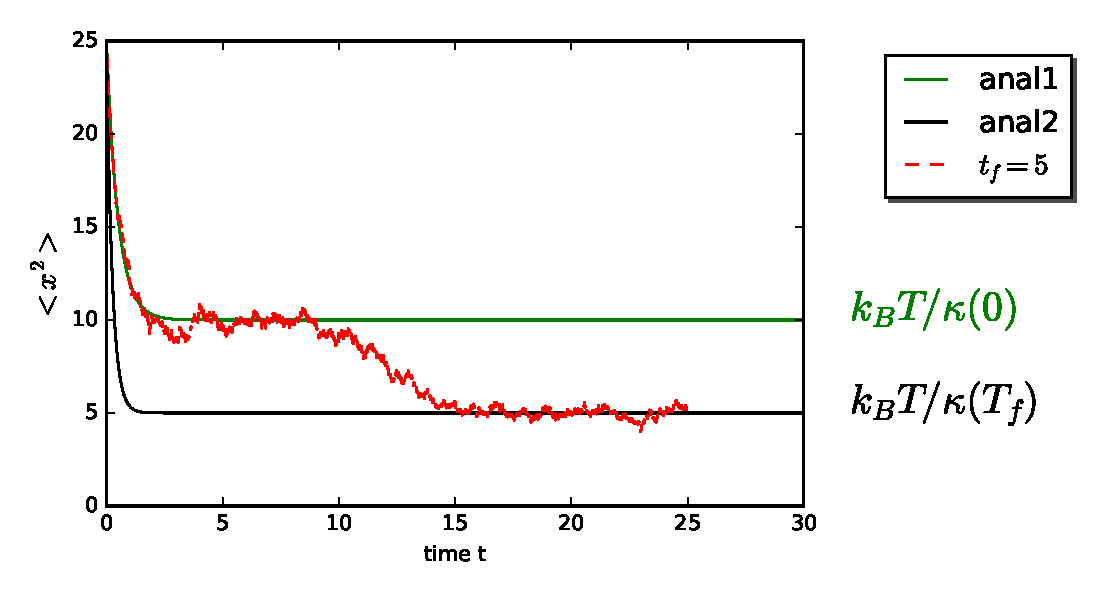
\includegraphics[scale=0.67]{ramp_anal.eps}
%\caption{ $\Delta t=0.001, D=10, \gamma=1$  and number of noise realizations $N_{exp}=1000$ over which it is averaged. }
%\label{sigma_ramp_anal}
%\end{figure}
%
%
%\underline{$\gamma=10$} \\

\subsubsection*{Linear ramp of spring's stiffness}


\begin{figure}[!htbp]
\centering
\includegraphics[scale=0.67]{ramp_protocol2.eps}\\
\caption{ Protocol of ramp with longer relaxation time}
\label{protocol_ramp2}
\end{figure}


The central idea is that we would be studying transition between two equilibrium configuration defined by spring constants $\kappa(0)=1$ and $\kappa(T_f)=2$ at initial and final time, respectively. Linear ramp of spring constant (figure \ref{protocol_ramp2}) is given by:



\begin{equation}
  \kappa(t)=\left\{
  \begin{array}{@{}ll@{}}
    1 & ,0< t <40 \\
    1+ t/t_f & ,  40 < t \leq t_f \\
    2 & , t_f \leq t \leq  t_f+ 40 \\
  \end{array}\right.
\end{equation}
where $t_f$ is the time it takes for spring constant to ramp from $\kappa=1$ to $\kappa=2$ and $T_f=t_f+40$ is the final time when we stop the numerical experiment. Thus, smaller the $t_f$, higher is the slope $ \dot{\kappa}=1/t_f$.  We have chosen 40 time units as the time interval that we give our particle to relax to equilibrium because numerically, we find that it relaxes to equilibrium before 40 time units. Hence, initially, with $\kappa(0)=1$, we give 40 time units for our Brownian particle to relax to equilibrium, and then after $t=t_f$ with $\kappa(t>t_f)=2$ , we again wait for 40 time units.

We have chosen $x(0)=5, D=10$ and $\gamma=10$. For all numerical calculations, $\Delta t=0.001$ and number of noise realizations $N_{exp}=1000$ over which it is averaged. 

When spring stiffness $\kappa =1$ is a constant for all time, we find mean position  $\langle x \rangle=5 e^{-t/10}$ (equation \ref{sol}). Further, mean position in all linear ramp protocols goes to zero after about 40 time units (figure \ref{ramp_mean2}).

\begin{figure}[!htbp]
\centering
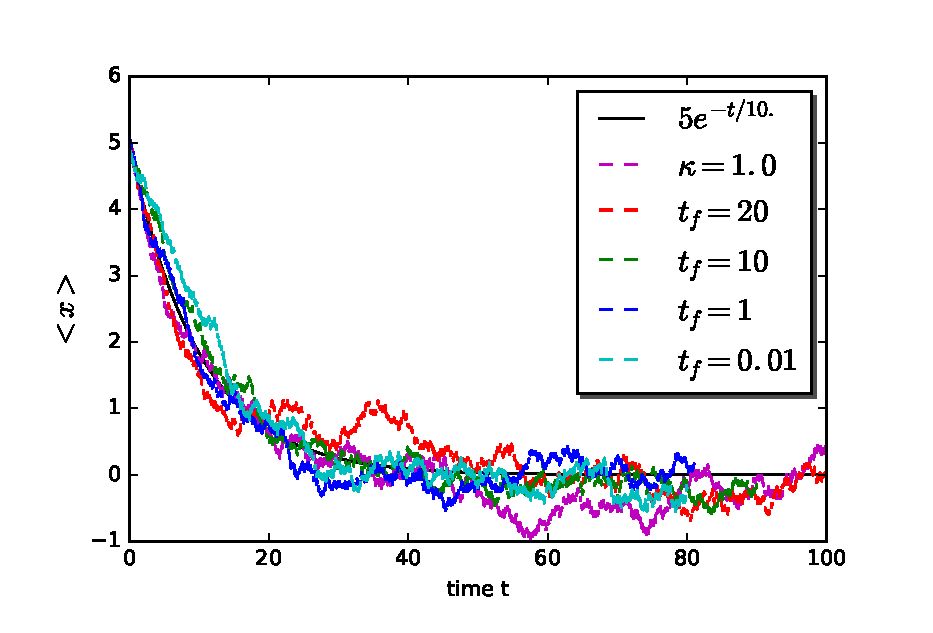
\includegraphics[scale=0.67]{ramp_mean2.eps}
\caption{ Mean position of Langevin particle under a linear ramp. $\kappa=1$ curve correponds to a constant spring stiffness for all time, and other curves are a function of $t_f$. }
\label{ramp_mean2}
\end{figure}

Similarly, when spring stiffness is a constant for all time, we find second raw moment of position to be given as (equation \ref{var_x}):
\begin{eqnarray}
\langle x^2  \rangle_1 &=& 25 e^{- t/5} + 100(1-e^{- t/5})\\
\langle x^2  \rangle_2 &=& 25 e^{-2 t/5} + 50(1-e^{-2 t/5})
\end{eqnarray}
where $\langle x^2  \rangle_1$ and $\langle x^2  \rangle_1$ is for $\kappa/\gamma=1/10$ and $\kappa/\gamma=1/5$, respectively. We note that after long time $\langle x^2 (t \rightarrow \infty) \rangle_1 =100 $ and $\langle x^2 (t \rightarrow \infty) \rangle_2 =50 $

Since relaxation time is  $\tau=\dfrac{\gamma}{\kappa}$, we have $\tau=5$ for $\kappa=2$ during time $t_f<t< T_f$.


\begin{figure}[!htbp]
\centering
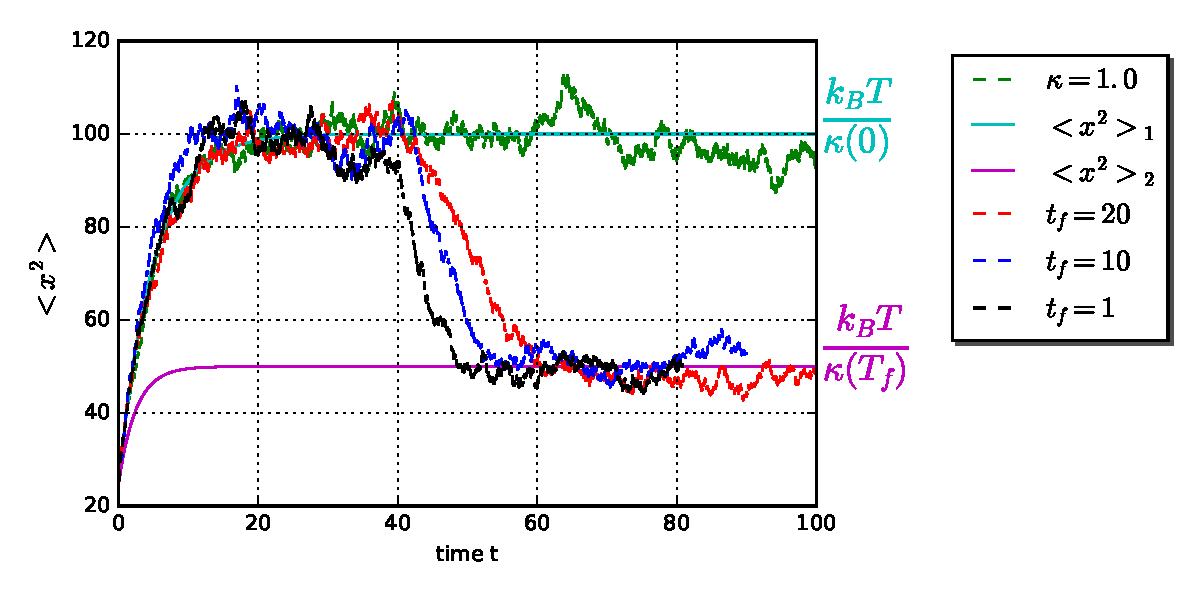
\includegraphics[scale=0.67]{ramp_sigma_gamma_10_first.eps}
\caption{Second raw moment of Langevin particle under a linear ramp. }
\label{sigma_ramp2a}
\end{figure}
 
On one hand, we find that when $t_f \gg \tau $, then Langevin particle goes from one equilibrium  state to another in the time $t_f$ in which the spring stiffness is increased from $\kappa=1$ to $\kappa=2$ (red line with $t_f=20 =4 \tau$ in figure \ref{sigma_ramp2a}). This is the limit, when the system is driven slowly. On the other hand, when the system is driven fast enough, then the Langevin particle is not able to keep up with the protocol and takes longer time to relax to equilibrium, which is of the order of $\tau$. This is the limit when $t_f$ is getting smaller compared to $\tau$. In this limit,  we find that Langevin particle starts taking longer than $t_f=1$ for this transition (black line with $t_f=1 = \tau/5$ in figure \ref{sigma_ramp2a}).

In figure \ref{sigma_ramp2b}, we see that no matter how quick the linear ramp is performed (smaller $t_f$), the Langevin particle takes almost the same amount of time to relax to the new equilibrium. 
\begin{figure}[!htbp]
\centering
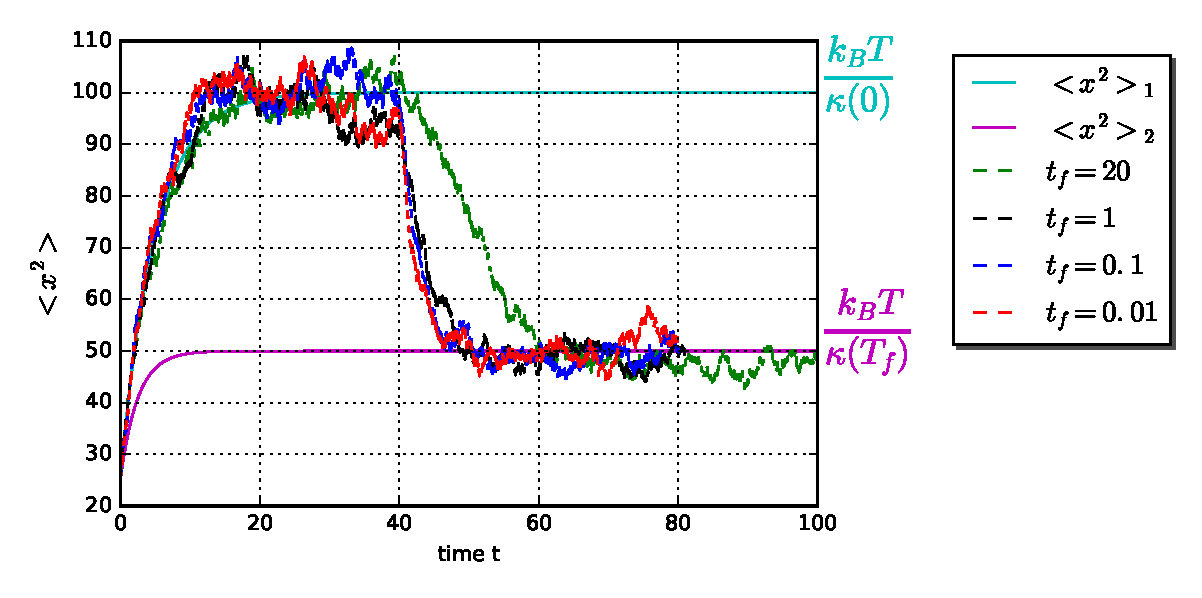
\includegraphics[scale=0.67]{ramp_sigma_gamma_10_second.eps}
\caption{ Second raw moment of Langevin particle under a linear \textit{quick} ramp with $t_f=1,1/10,1/100$. }
\label{sigma_ramp2b}
\end{figure}



\section{Fokker-Planck dynamics}
When we average over position over all noise realization, we get Fokker-Planck equation. It describes the time evolution of  probability distribution of position. 
\subsection*{Random walker}
We expect that the probability of a random walker should be a guassian with zero mean and a variance growing linearly in time. Let's derive it from Fokker Planck equation. 
\begin{equation}
\dfrac{\partial \rho}{\partial t} =  D \dfrac{\partial^2 \rho}{\partial x^2} 
\end{equation}
We assume that the random walker initially was located at origin, i.e. $\rho(x,0) = \delta(x)$. Then, we get $\rho (x,t) = \frac{1}{\sqrt{4  \pi D  t}}e^{-{x^2}/({4 Dt})}$ 

By comparing it with the standard form of guassian distribution $P(x)= \frac{1}{\sqrt{2\pi\sigma^2} } e^{ -\frac{(x-\mu)^2}{2\sigma^2} }$,  we can find mean $\mu$ and variance $\sigma^2$. It matches with what we got in Langevin dynamics, i.e.  $\langle \Delta x\rangle=0$ and $\langle \Delta x ^2\rangle=2 Dt$, where $\Delta x= x(t)-x(0)$ \footnote{ For the wavefunction of free quantum particle, the Schr\"odinger equation looks exactly the same as the above classical diffusion equation. Now in that case, we find $\langle \Delta x_Q ^2\rangle \sim t^2$. Why it's different? It's because Schr\"odinger equation involves quantum probability amplitude $\psi(x)$, not probability $|\psi(x)|^2$. The variance of  complex-valued $\psi(x)$ does spread linear in time, but that's different from quantum variance of position which grows quadratically in time as the later is computed from quantum probability. Hence, for quantum free particle $\langle \Delta x_Q ^2\rangle = \int   x^2 P_Q(x,t) dx=  \int   x^2 |\psi(x,t)|^2 dx \sim t^2$ and for classical diffusive particle $\langle \Delta x_C ^2\rangle= \int   x^2 P_C(x,t) dx \sim t$. } .



\subsection*{Overdamped Brownian particle}
Fokker-Planck equation for the overdamped Brownian particle in Harmonic potential would have an additional term :
\begin{equation}
\partial_t \rho=  \partial_x \left( \dfrac{\kappa(t)}{\gamma} x \rho \right) + D \partial_{xx} \rho
\end{equation}
We would find that the equilibrium distribution would be again a guassian, whose variance would be linear in temperature \footnote{This can be compared with variance of random walker which is linear in time.} .

For our problem of transition between two equilibrium states, probability density $\rho$ should be constant both at initial and final time. For time $t=0$, we get:
\begin{eqnarray*}
 D \partial_{xx} \rho+  \partial_x \left( \dfrac{\kappa(0)}{\gamma} x \rho \right)  &=& 0 \\
  \partial_{xx} \rho + \alpha( x \partial_x   \rho +  \rho) +   &=& 0
\end{eqnarray*}
 where $\alpha = \dfrac{\kappa(0)}{D \gamma}= \dfrac{\kappa(0)}{k_B T}$, using fluctuation-dissipation relation.
We find that $\rho(x)= A e^{-\alpha x^2/2} $, where $A$ is a normalization constant, satisfies the above equation. Hence, we note that variance $1/\alpha \propto T$. Similarly, at time $t= t_f$, we find that particle's probability density $\rho$ is a guassian with $\alpha = \dfrac{\kappa(t_f)}{D \gamma}=\dfrac{\kappa(t_f)}{k_B T}$.

We find that mean of distribution is zero and it's variance is constant in time, and linear in Temperature. This matches with what we had obtained from Langevin dynamics of overdamped particle in long time limit. 
\section{Thermodynamics calculation}
\subsection*{Hamiltonian}
Our model is an open classical system. It is in canonical ensemble where our Brownian particle is in contact with heat bath of temperature $T$. The affect of heat bath on the particle is two-fold: reducing the energy through dissipation and giving kick with a random force through noise term.

Hamitonian of the total system $H_t$ is 
\begin{equation}
H_t = H_b + H_s + H_{int}
\end{equation}
where $H_b$, $H_s$, $H_{int}$ are the Hamiltonian of bath, system and interaction between bath and system. If we follow standard statistical mechanics, heat bath would be weakly interacting so that we can ignore $H_{int}$ term. Heat bath defines temperature $T$ and we get partition function as $ Z= \int d\Gamma e^{-\beta H}$, where $\beta$ is inverse temperature and $d\Gamma$ is infinitesimal phase space volume $dpdq$.

Let's write the Hamitonian of the system generally. We would ignore the noise and dissipation term in equation \ref{eom} since it's because these terms are the effect of bath on the system.
\begin{equation}
H_s = \dfrac{p^2}{2m}   +\dfrac{1}{2} \kappa(t) x^2
\end{equation}

For writing the Hamiltonian of system $H_s$ of our overdamped Langevin particle,  we should ignore kinetic energy term, and for underdamped we should ignore potential energy. Essentially, we are comparing which component of energy is bigger

 %\footnote{This nomenclature as defined in literature \footnote{include reference} is misleading if we compare it to textbook problem of damped harmonic oscillator. In the old problem, we would compare dissipation with product of mass and spring constant term.}.

The Hamiltonian of system $H_s$ of our overdamped Langevin particle \footnote{Trouble is that this doesn't give us correct equation of motion \ref{eom}. But for now, we would go ahead because this hamiltonian does gives the free energy difference that matches exactly with that given in \cite{martinez2016engineered} }
\begin{equation}
H_s = \dfrac{1}{2} \kappa(t) x^2
\end{equation}


At time $t=0$ and $t=t_f$, our particle is in equilibrium. Hence, we can find thermodynamic quantities like free energy, partition function, entropy and internal energy. Let's find partition function because other physical quantities can be derived from it.

\subsection*{Partition Function}
Let's denote $\kappa(0)= \kappa$. Since, over-damped particle has a single degree of freedom $x$, we have partition function $Z$ given by:
\begin{equation}
Z = \int dx e^{-\beta H}= \int dx e^{-\beta \kappa  x^2/2 \gamma}= \sqrt{\dfrac{2  \pi}{\beta \kappa}}
\end{equation}
Hence, we have free energy $F = -k_B T \ln Z=-\frac{k_B T}{2} \ln \dfrac{2   \pi}{\beta \kappa} $. This means free energy difference between two equilibrium states will be $\Delta F =\frac{k_B T}{2} \ln \dfrac{\kappa(t_f)}{\kappa(0)} $. This matches with the expression of free energy difference given in \cite{martinez2016engineered}.

Now let's talk about internal energy. $U= \langle E \rangle = \frac{k_B T}{2}$, which is the statement of equipartition theorem. Since the temperature is the same, $\Delta U=0$.
\begin{eqnarray*}
 F&=& U-TS\\
 \Delta F &=& \Delta U-T \Delta S \\
  \Delta F &=& -T \Delta S \\
  \Delta S &=& - \Delta F/ T= -\frac{k_B}{2} \ln \dfrac{\kappa(t_f)}{\kappa(0)} 
\end{eqnarray*}

\subsection*{Work done}
$\langle W \rangle= \int dH = \int \dfrac{\partial H}{\partial \kappa} d\kappa= \int \langle x(t)^2 \rangle \dot{\kappa} dt$


Hence, we note that work done for constant spring stiffness is zero. For linear ramp protocols, we get $W \propto 1/t_f$. Hence, shorter the time interval $t_f$ is, bigger is the work done.

\appendix

\section{Model with velocity degree of freedom}\label{sec.vel_dof}
Let's write the general equation of a particle with dissipation $\gamma$ and noise term $\xi$:
\begin{equation}
m \ddot{x}= -\gamma \dot{x} + \xi(t)
\end{equation}

We would focus here on dissipation that is proportional to velocity as we have already studied the other model where dissipation proportional to position. Like before, to understand the affect of noise and dissipation, we would first study two subcases: random walker (one with only noise term) and tired walker in velocity(the one with only dissipation term). 





\subsection*{Random walker in velocity space: affect of noise}
Langevin equation for a random walker in velocity space (with $m=1$) is given by:
\begin{equation}
\dot{v}=  \xi(t)
\end{equation}

We find that  $\langle \Delta v\rangle=0$ and $\langle \Delta v ^2\rangle=2 Dt$, where $\Delta v= v(t)-v(0)$.


\subsection*{Tired walker in velocity space: affect of dissipation}

If there is no spring constant $\kappa$, then  we find that we get dissipation in velocity:
\begin{equation}
\dot{v}=  - \frac{\gamma } {m}v 
\end{equation}
We get $v(t)=v(0) e^{-\kappa t/\gamma}$ as solution. It means as $t\rightarrow \infty$, speed (and position) of particle goes to zero no matter what is the initial velocity (and position). Here, dissipation takes away kinetic energy of the system. 

\subsection*{Brownian particle}
Now let's consider Brownian particle with dissipation constant $\gamma$ and noise $\xi$ term together. It follows:
\begin{equation}
\dot{v}= -\dfrac{\gamma}{m} v + \xi(t)
\label{eom_vel}
\end{equation}




We get equation of motion to be similar to what we obtained before with position $x$ replaced by velocity $v$.
\begin{equation}
v(t)= v(0) e^{-\gamma t /m} + \int_0^t ds  \xi(s) e^{-\gamma (t-s)/m} 
\label{sol_vel}
\end{equation}

\begin{equation}
\langle v^2 (t) \rangle = \langle v^2 (0) \rangle e^{-2\gamma t /m} + \dfrac{D \gamma}{m}(1-e^{-2\gamma t /m})
\label{var_vel}
\end{equation}

As derived in class, second raw moment of position $\langle \Delta x^2 (t) \rangle$ is given by:
\begin{equation}
\langle \Delta x^2 (t) \rangle = 2 \dfrac{k_B T}{\gamma}\left[t-\dfrac{m}{\gamma} +\dfrac{m}{\gamma}e^{-\gamma t /m} \right]
\end{equation}
Since $\langle \Delta x^2 (t) \rangle= 2 D t$, we get $D=\dfrac{k_B T}{\gamma}$

\section{Euler-Maruyama algorithm}\label{sec.Numerics}
We have used Euler-Maruyama algorithm to study Langevin equation numerically. Let's write the Langevin equation as follows:
\begin{equation}
\dot{x}= -\Omega x + \xi(t)
\end{equation}
Now as discussed before, the main issue is how to simulate white noise $\xi$ numerically. 
I find that it's best explained in \cite{ladd2015numerical}. Now I will quote discussion from \cite{ladd2015numerical}  without any changes:

`` In the literature of stochastic differential equations (SDE’s), for example the excellent book by Kloeden and Platen , the SDE is written in incremental form:
\begin{equation}
dx_t= -\Omega x_t dt + \sqrt{2D} dW_t
\end{equation}
where $D \propto T$. The term $dW_t$ is an increment of a Wiener process $W_t$ , which is a piecewise continuous function that is most simply described as a succession of random increments, 
$W_{t_1} ,W_{t_3} W_{t_3}$. Each increment $dW_{t_i}= W_{t_{i+1}}- W_{t_{i-1}}$ is sampled from a normal distribution with zero mean and variance $t_{i+1}- t_{i}$. The properties of a Wiener process can be summarized in the following relations:
\begin{equation}
W_0=0, \langle W_t\rangle=0, \langle (W_t - W_s)^2\rangle=|t-s|
\end{equation}

Euler-Maruyama algorithm is given by 
\begin{equation}
x_{n+1}= x_n (1 - \Omega \Delta t) + \sqrt{2 D \Delta t} \phi_n
\end{equation}
where $\phi_n$ is a guassian distribution with zero mean and unit variance."

\bibliography{ref} 

\bibliographystyle{plain}

\end{document}